%   MSc Business Analytics Dissertation
%
%   Title:     Aaa Bbbbbbb Cccccccccc
%   Author(s): Xxxxxx Xxxxxxxxx and Yyy Yyyyyyyyy
%
%   Chapter 3: Literature Review
%
%   Change Control:
%   When     Who   Ver  What
%   -------  ----  ---  --------------------------------------------------------------
%   11Feb11  AB    0.1  Begun 
%

\chapter{Literature Review}\label{C.LitReview}
\section{Introduction}\label{S.intro3}

In recent years, purchasing capability of an \textbf{economy} has increased due to improvement in their finances, and employment levels. Ranging from buying small household items to\textbf{ expensive items such as a house, a car or an office}. To buy a house or a car, one needs to have a large amount of money available to him; that is not necessarily possible most of the time. \\

\textbf{Start with an exmaple to explain what is loan}. There are certain critical circumstances that can occur anytime, where one may need a certain amount of cash. So one may need to borrow a generous amount of money from some other entity which is called a loan. A loan is lending a sum of money from one entity to another that involves repayment of the amount in near future. Lent amount is called principal amount and amount to be repaid is a summation of principal amount and an interest amount or other charges. It is not as easy as it sounds like, there are certain terms need to be agreed upon by each entity before exchange of the money. A loan can be for an amount taken at one time or can be taken in instalments {Partial Payments]. A loan can be provided by banks, corporations and financial institutions. Banks and financial institutions provide various types of loans as per the need of an applicant, such as personal loans, home loans, business loans, credit card loans and cash advances. There are times when the borrowing amount is very large and banks cannot provide the loan based on verbal agreement, they need to ensure that if an applicant is not able to repay the loan then they need to have a source to recover the lent amount. So, in this case, an applicant needs to apply for a mortgage with the bank.\\

A mortgage or collateral is an instrument that applicant has to pay back with predefined series of payments to the bank and financial institutions. Over a duration of time, an applicant needs to repay the loan inclusive of interest amount in order to free his/her mortgage. In case, if an applicant is not able to repay the loan within predetermined time, then the bank can recover their money by selling or putting it for auction the mortgage. The most common type of mortgage is residential mortgages were applicant gives his/her house to banks and in a case of no repayment then a bank will claim the house to recover the balance amount of the loan. This will give a bank a security that their lent amount is not at risk and over the years they will get back their lent money one way or the other. Mortgages come in various different forms. Most commonly used mortgage types are Fixed Rate Mortgage where applicant repays the loan amount on a fixed rate throughout the period determined and Adjustable Rate Mortgage where interest rate varies as per the changes in market interest rates. Our work is based on analysis of residential mortgages with varied interest types which will be discussed in later sections.\\

Put \textbf{Photo of loan application process folw chart}

Before analysing data based on residential mortgages, one needs to understand the process of giving a loan. Depending upon the requirement an applicant applies for a loan by filling an application form with all the necessary details required by the bank. Bank officials then analyse the application and may ask an applicant for additional information; after evaluation, bank approves or disapproves the loan. Next, borrower and bank sign an agreement that states all the terms and conditions of the loan including determined interest rate and type of mortgage. Lastly, loan amount will disburse and borrower will start repaying the instalments that constitute principal amount and interest amount for predetermined period of time.\\

And, the major question is how do banks decide whether to give a loan or not? This question is of major concern as bank's cash flow highly depends on timely repayment of the loan. Every bank does not have the same procedure but majority of the loan review process is same. Following are few characteristics that bank officials will concentrate while evaluating a loan application:
\begin{enumerate}
	\item Credit history of applicant
	\item Loan to Value ratio
	\item Employment history
	\item Character assessment of applicant
	\item Evaluation of collateral
	\item Financial statements such as bank history, cash flow, etc. 
\end{enumerate}

\section{What is Credit Scoring?}\label{C.risk}
One of the most important questions of borrowing and lending process of loan is How do banks make sure whether to give a loan to a borrower or not? Banks do credit evaluation of an application to make credit management decisions. Officials collect, analyze and classify credit variables and elements to reach credit decisions. Credit evaluation determines the quality of the bank. A process of evaluating customer's bad credit risk is called credit scoring. Since ages, there have been various definitions of credit scoring; \citet{hand1998consumer} stated that credit scoring is a process of measuring customer's credit-worthiness. \citet{anderson2007credit} segregated credit scoring into two components: credit that means you can purchase now and repay the amount later; and, scoring means ranking based on predefined set of qualities to differentiate amongst cases to achieve credit decisions. On the other hand, \citet{gup2005commercial} stated that process of credit scoring uses statistical approaches to determine whether a borrower will default in future or not. Similarly, \citet{beynon2005optimizing} said, credit scoring is a statistical model that convert relevant credit data into numerical data that support credit decisions.Credit scoring techniques have been widely used to access commercial loans, businesses, real estate industry and residential mortgages \citep{gup2005commercial}. Credit scoring is a method that decides whether an applicant will get credit, what will the process of getting credit and how will the strategies enhance borrower's profitability. Credit scoring models are prevalent from last ten decades that has evaluated consumer credit secure and reliable \citep{thomas2002credit}. 

\subsection{Traditional Subjective Assessment System and Credit Scoring}\label{C.risk2}
The primary objective of credit evaluation process is to compare and contrast characteristics of an applicant with other previous candidates who have repaid the loan amount. Bank will check candidate's profile with earlier candidates, if a profile is very much similar, then they will check if an applicant has repaid the loan on time. If a claimant did not default then the loan can be granted, if not then loan application will be rejected. \citet{crook1996credit} stated that there are two techniques for credit evaluation: Credit Scoring and Officials Subjective Assessment. Traditional judgement assessment method is entirely dependent on evaluator's experience and knowledge \citep{sullivan1981consumer,bailey2004consumer}. Subjective assessment is subjective and inconsistent, but on the other hand it can be successful, creditor's experience can be qualitative that helps in taking successful credit decisions.\\

While in credit scoring method, creditors use their knowledge and historical information of the loan applications to form an evaluation model to determine creditworthiness. Credit scoring methods are consistent, and self-operated that includes quantitative measurements of applicant's credit score subjected to predictor variables such as employment duration or credit history. Also, credit scoring method provides an advantage to a bank to keep their good credit customers intact and to improve customer service. Consequently, this process has been criticized because data that has been used consists of some assumptions to evolve model statistically.\\

\subsection{Advantages and Disadvantages of Credit Scoring}
In \citep{crook1996credit}, Crook said that credit scoring process does not require too much information because the process the model has been statistically developed for a particular set of variables; on the other hand, subjective assessment does not have any variable reduction method because of no statistical importance. Credit scoring method reduces bias by inspecting rejected applications; it will keep score how rejected applicants would have behaved if they have given the loan. It considered both good and bad credit players and built a model on a large number of applications compared to traditional methods. Scoring models also contain a significant number of relevant variables that show a correlation between variables and payment behavior. A significant advantage of this approach is its reusability; the process can be used multiple time over the same data set with accuracy. Scoring models reduce processing cost and time with efficiency and ease decision-making process.\\

But, at times credit scoring model can inaccurately predict the creditworthiness of an applicant because of misclassification error. Due to its variable reduction technique, a model can miss out important variables to evaluate application which can be necessary. There may be chances that an applicant can repay the loan on time but based on the historical data or any missing information; a model can predict the wrong result. Also, these model can not be standardized as each industry can have different credit scoring models. Historical data can play a disadvantage as due to advancements in technology and rapid changes in economic factors, credit score model prediction can be inaccurate. Models are standardized and need to update as per the economic factors, that can cost much, and the process is not easy. 

\subsection{Is credit scoring process optimal?}\label{C.optimal}
\citep{al2002credit} Despite so much criticism on credit scoring models performance, credit scoring models are in use; but, there are some open questions which have left unanswered: Optimal evaluation of an applicant, relevant variables to evolve a model, information needed to enhance decision making, best measures that can predict loan accuracy, extent to which an applicant can be classified as defaulter.\\

Contrast to \citet{al2002credit} questions, \citet{abdou2009credit} added more open questions to credit scoring process: How to choose appropriate technique to perform classification? Are there any other better classification methods better than credit scoring method? Is predicted value of the credit scoring model efficient than other methods? How to find out appropriate factors that influence credit scoring?\\

As mentioned above that credit risk majorly enhance bank's quality in spite of economic and environmental changes. So banks need to have suitable methods to evaluate credit risk. A good system should be able to correctly classify between good and bad credit customers because bad credit could cause some severe issues to the bank. Our work will discuss few techniques that can be used to evaluate credit risk by determining a probability of default and classification of chances of default. Also, our work will try to find out techniques that can enhance the assessment and analysis process of the credit.

\section{Analysis and assessment of credit}\label{tech.crisk}

Importance of assessing credit worthiness has been increased since, the property crash in 2008. Banks and Financial instituions making efforts to enhace tranditional credit scoring mechanisms by incorporating latest technology and tools. Not only avaiablity data about customer but also rapid development in machine learning and analytics providing a foundation stone to banks. \\

Traditional credit scoring process with random selection of good and bad portfolio from creditors file around 50 - 300 \citet{capon1982credit} chartartestics points from loan portfolios to build a essential subset to perform statastical analysis. In \citep{10.2307/2983268}, Hand mentioned about three commonly used approaches used for selecting characterstics out of avialble data: Expert Knowledge, Stepwise Statstical procedure and evaulating individual characterstics. Subject Matter Expert(SME) \\

Credit analysis and assessment is very important for banks and financial instituions to evaluate the credit worthiness of an applicant or a borrower. Banks implements various factors while assessing credit risk; such as credit rating, loan to value ratio, probability of default, etc.; that leads to derivation of credit risk rating. Variety of financial techniques have been used by the officials to analyse credit risk.\\

An applicant credit score is generated using credit rating system based on various charterstics points. Thereafter credit score is used depending on the usage of system. There are single cut-off and two cut-off stages in deciding application decision. In single cut-off, credit is granted if applicant score is higher than cut-off; otherwise credit is denied. Some instituations incorportae two stage cut-offs, in this system if credit score is higher than upper cut-off then credit is granted straighted and denied if score is lower thant lower cut-off. If score is between upper and lower cut-off then applicant credit history is pulled to calculate further scoring point and added to credit score. If new total score is higher than upper cut-off then credit is granted else denied.\\

Banks and financial instution sets their own cut-off for credit score based on the probablities of each applicant ability to repay or nonpayment of credit amount.\\

Adding flow chart of Evaulation Process and Pricing
\begin{figure}
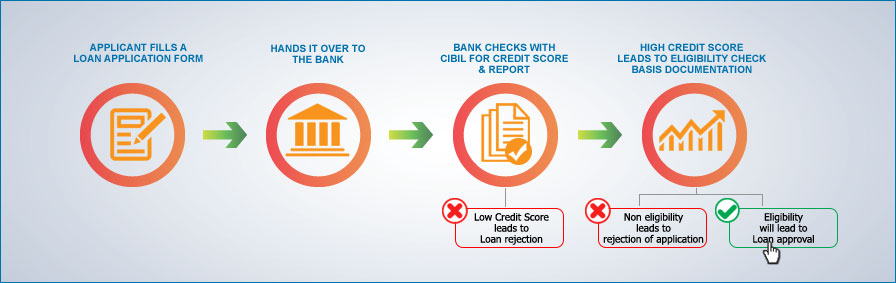
\includegraphics[width=\textwidth]{creditscoreflow.jpg}
\end{figure}

However, Credit Risk has recevied a lot of critisim as well from Academics and Researchers. \citet{al2002credit} has questioned about optimal method to evaulate customers? What are key variables or data points which an analyst must consider while evaulating customer applications? On what basis one can classify an applicant as good or bad?\\


However, apart from above questions following can be useful when building a new credit scoring system. One should evaluate statistical techniques or algorithm by its accuracy to correctly classify historical portfolios into good or bad credit from creditors file. Also, Banks and Financial institution's identified factors that can influence the prediction of credit and loan quality by gathering all possible information from customer applications form, bank transactions history and previous credit history. Credit Analysts analysis of all these information to decide what all variables or characteristics to be included in final the credit model.\\


One of the principal objectives of credit scoring system is to assist Banks and Financial Institutions to streamline their credit management procedure and policy that will enable analysts with an efficient tool which will provide fast and accurate analysis of credit.On the longer run, such tool helps banks to avoid bad credit and scale up bank revenues and profit by selling more financial products to customers.\\


\section{Diffrrerent Technology in Credit Risk:}


% Please add the following required packages to your document preamble:
% \usepackage{booktabs}

\begin{table}[!ht]
\centering
\caption{Different Statistical Algorithms for Credit Scoring}
\label{my-label}
\begin{tabular}{|p{3cm}|p{10cm}|}
\toprule
\textbf{Method}                & \textbf{Authors}                                                                                                                                                       \\ \midrule
Linear Regression     & \cite{lee2005two,10.2307/2983268}                                                                                                                          \\
Discriminant Analysis & \cite{fisher1936use,durand1941risk,altman1968financial,eisenbeis1978problems,zhou2016research,liberati2017advances}                                        \\
Logistic Regression   & \cite{hosmer1989best,altland1999regression,nie2011credit,abdou2008neural,bensic2005modelling,joanes1993reject}                                             \\
Decision trees        & \cite{kohavi2002data,breiman1984classification,zhang2010vertical,zekic2004small,zhou2008new,huang2007credit,xia2017boosted,koh2015two,koutanaei2015hybrid} \\
Neural networks       & \cite{demuth2008neural,west2000neural,gately1995neural,presky1996functional,ghosh1994credit,desai1996comparison}                                           \\ \bottomrule
\end{tabular}
\end{table}
\textbf{Linear Regression} allows one to build to simple model using a dependent and two or more predictor data points, and it is being used in credit scoring models as the two class problems can be represented using a dummy variable \citep{lee2005two}. A Poisson regression can be used to classify cases where customer tends to partial repayments, and these payments can represent as a Poisson count in the model. Credit analysts can promptly analyse using linear regression credit model to investigate customer factor such as past payments record, credit guarantees and default, etc. against a predefined cut-off credit score. If new applicant credit score is higher than cut-off score, then credit is granted \citep{10.2307/2983268}.\\

\textbf{Discriminant Analysis:} In credit scoring models,  a statistical analysis method called Discriminant Analysis is regularly used by the researcher to rapidly build a prototype model when there are two or more categorical dependent variables for analysis. Multiple Discriminant Analysis(MDA) utilised in various studies and business verticles for the variety of applications since its inception in 1930's \citep{fisher1936use}. \citet{durand1941risk} used the Discriminant analysis for modelling a scoring system that gives a prediction about loan repayment. Many researchers agreed that the MDA is the best use to classify a group of categorical variables into two or more predictor or classes. For example, Credit Analyst can build a scoring system using MDA to categorised a new loan application into Default or Non-Default category, and this will help banks to avoid those applicants who have potential to default in repayment sooner or later.\citet{altman1968financial} used MDA by developing a scoring model based on five financial ratios by analysing financial statements to select eight variables for predicting financial bankruptcy in Corporates. \citet{eisenbeis1978problems} noted the problem associated with Discriminant Analysis such as reduction in dimensionality, improper estimation of classification error, using linear functions instead of quadratic functions, etc. Despite these limitations in MDA, it is still one of the techniques which are often used by credit analyst in building credit scoring system \citep{zhou2016research,liberati2017advances}.\\


\textbf{Logistic Regression} has resemblance with Linear regression and it is also most commonly used statsical technique for building credit scoring system. Dichtomous nature of logistic regression outcome probablity (good credit or bad credit) makes it different from linear regression. \citep{hosmer1989best}. By using two or more independent variables, one can build the simple logistic regression model. However, logistic regressions with more than one independent variables use the maximum likelihood method to build credit scoring model.\citep{altland1999regression}. Logistic regression has been widely used in building credit scoring system in financial domain ( see for example: \citep{nie2011credit,abdou2008neural,bensic2005modelling,joanes1993reject}) \\


\textbf{Decision trees} is one of the classification techniqeue in machine learning and widely using for buidling credit scoring system. Classification \& Regression Trees (CART) and C4.5 are two widely use decision tree algorithms \citep{kohavi2002data}. One of the firts model pioneered by \cite{breiman1984classification}.
\begin{figure}
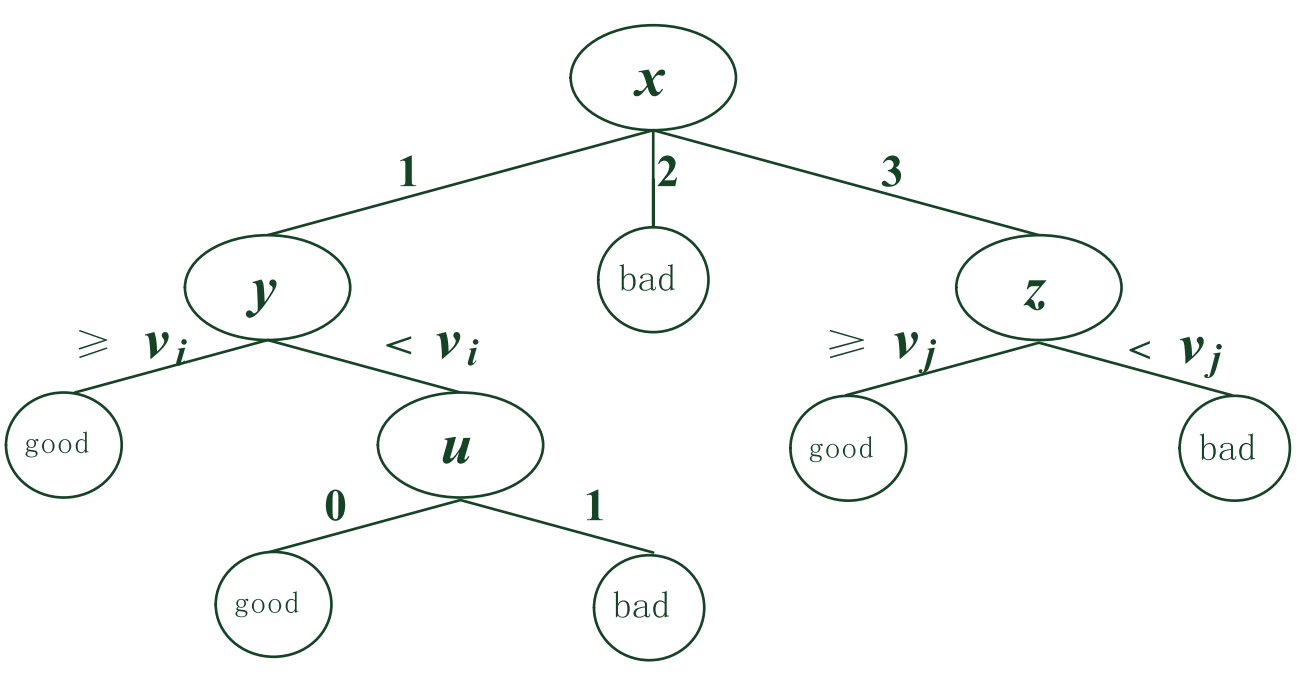
\includegraphics[width=\textwidth]{simpledt.png}
\caption{Simple Decision Tree 
Source: \citep{zhang2010vertical}}
\end{figure}
With the help of single input function, algorithm splits all data observations to generate a dichotomous tree using CART.  The algorithm chooses the best subset data based on the lowest cost of misclassifications\citep{zekic2004small}. This process of selecting attribute from data subset is repeated as algorithm C4.5 or CART continues to choose one attribute that splits data into subset based on information gain \citep{zhou2008new}. \citet{huang2007credit} used decision tree along with support vector machines to build credit scoring model. Other applications on using decision tree in credit scoring has been discussed by \citep{xia2017boosted,koh2015two,koutanaei2015hybrid}.\\


\textbf{Neural networks} in machine learning or data mining is modelling system, which is based on the human brain and nervous system. A Neural network consists of several neurons(nodes) connected to determine the functionality of the network \citep{demuth2008neural}. \citet{west2000neural} carried out several experiments to measure the performance five different types of the neural network for credit scoring. While conducting experiments, \citet{west2000neural} observed that Logistic regression is slightly more accurate in prediction in comparison to neural networks. This Research also noted that CART and \emph{k} Nearest Neighbour results are not par with logistic regression. The neural network requires being trained on a dataset to predict the outcome of decision variables correctly \citep{presky1996functional}. In 1996, \cite{gately1995neural} discussed applications of using the neural network in financials domains such as fraud detection in credit card transactions, forecasting company bankruptcy, classifying bad or good loan application and others areas where neural networks are successful\citep{ghosh1994credit}. \citet{desai1996comparison}, compared the performance of a neural network and logistic regression and found that neural network able to correctly predict loan portfolio when the measure of success is accurately classifying bad loans only.

\section{Geospatial}

Geospatial data is a dataset which contains or provide information about geographical location/s. To analysis geospatial data, one requires a system that can interpret and process geographic data about latitude and longitude and assist decision makers in providing insights out of that data. Such systems are called Geographical Information System \citep{keenan1998spatial}. In recent years,we have seen rapid enhancement in the technology as a result the amount the spatial data available from stateliite and user mobile data has been growing.\\

In \citep{can1998gis}, Can said that for housing and mortgage spatial data is a critical aspect as housing information remain as is in geographical space. In credit scoring system, one can combine spatial information of a particular location such as employment, property value, property area, average income, etc., with financial data to build a robust predictions model.citep{can1998gis}, also noted that geospatial data is important for any business and policy, still its usability in mortgage and credit assessment is limited. In recent years, some researchers attempted to incorporate spatial data to estimate house prices\citep{tse2002estimating}, \citet{carling2005asymmetric} combined the geographical information with loan data to examine the credit rationing.\\

Availablity of high-end GIS software and fast computing environment makes it easier to utilise its power to strength credit scoring model along with the machine learning. By doing this not only bank and financial institutions to monitor or predict bad loans based on location, but also enable them to make new business strategies to reach out to uncovered audience or market.

\section{Data Visualisation}

Data volume has been increasing day by day and it has become difficult to analyse the data at once using tables and reports. And it is known that human brain retains more information, when it is received visually. Therefore, need for visual analytics has been increased from last few years and is growing rapidly. Data visualisation helps understanding complex data visually by easy pattern recognition, trends and provides granularity.\\

Data volume has been increasing day by day, and it has become difficult to analyze the data at once using tables and reports. And it is known that human brain retains more information when it is received visually. Therefore, need for visual analytics has been increased from last few years and is growing rapidly. Data visualization helps understanding complex data visually by easy pattern recognition, trends and provides granularity. Data visualization also helps a user to play with data by making alterations. It also provides ease of improvement, classification of relevant factors that can enhance consumer behavior, easily predict sales trends and customer behavior.\\

Data visualization tools such as Qlik, Tableau, R Shiny have played a significant role in demonstrating analytics and driving data insights to the users. Such tools are easy to operate compared to traditional statistical tools and software; that has led to enhancement in Business Intelligence. To explain results of advanced analytics and predictive algorithms to all users, it is essential to present the results to maintain performance visually.\\

Residential mortgages data consists of the geographical distribution of house locations. \citet{sun2013web} stated that data visualization analyses and quickly derive stories efficiently and interactively. Organizations are extensively using data visualization tools; as this software support drilling down the information and filtering the data as per requirement. Such software provides a facility of combining all the required information on a single platform called dashboard. Data visualization supports Geo spatial data very well, and our work is primarily dependent on geographical locations of residences. Our work focuses on combinations of longitudes and latitudes that helps in identifying exact address of a house.\\

Because of the high volume of geospatial data, it is important to maintain latency between residential data and output generated by predictive models. For the reasons as mentioned above, data visualization is essential for our work that will help to visualize the results for the end users.



\subsection{Examples of citations}\label{SS.citations}

In \citep{Atiyah:1961,Atiyah:1966a,Atiyah:1966b}, Atiyah builds on the work of \citet{Adams:1962} to develop 
the foundations of topological $K$-theory.  \citet{LewMcG:2000} and \citet{McG:2002} later extend parts of 
this to a previously unexplored algebraic setting.
